As previously stated, the game belongs to the space shooter genre. Such games involve the control of a space ship, flying in a two-dimensional or three-dimensional space, avoiding collisions with other spatial bodies by dodging or shooting the ship weapon(s) at the targets. Generally, such a game includes ``life'' mechanics, such that the player ship will eventually be destroyed and the game ended upon taking too much damage. \\ \\
Because the purpose of this game is purely demonstrative with regard to performance optimization techniques, certain irrelevant or negligible components are missing. As such, the game has no clearly defined goal / victory conditions, nor does it implement any game control mechanics beside a simple defeat screen. The game also does not have any sound effect, as a full study on all features present in Unity would not be feasible in the context of this study. Menus are limited to the defeat screen, enabling the player to restart the game. \\ \\
The game assets (models, textures, effects) have been either made from scratch, imported from the Asset Store with usage rights or imported and modified.
\begin{figure}
\centering
\begin{subfigure}{0.49\textwidth}
\centering

\begin{subfigure}{0.49\textwidth}
\centering
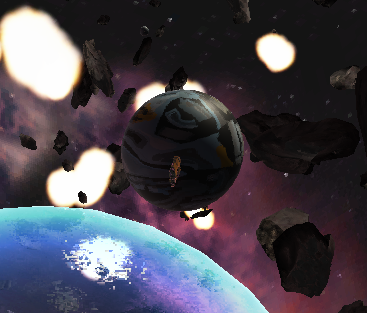
\includegraphics[width = \textwidth, height=\textwidth]{images/game1}
\caption{Space Drone - hostile}
\label{fig:top}
\end{subfigure}
\begin{subfigure}{0.49\textwidth}
\centering
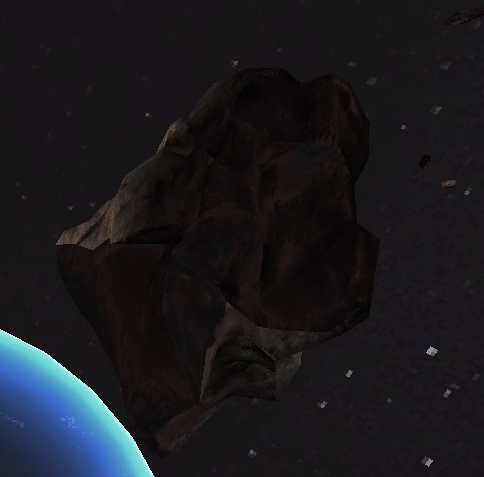
\includegraphics[width = \textwidth, height=\textwidth]{images/game2}
\caption{Space Asteroid - passive}
\label{fig:bottom}
\end{subfigure}

\label{fig:left}
\end{subfigure}
\begin{subfigure}{0.49\textwidth}
\centering

\begin{subfigure}{0.49\textwidth}
\centering
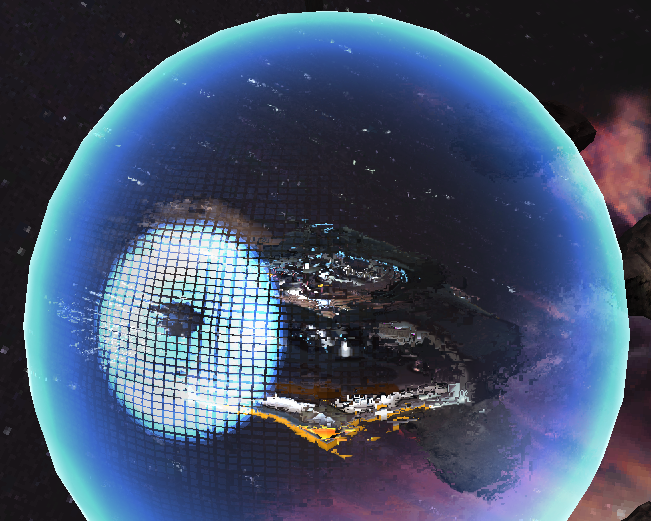
\includegraphics[width = \textwidth, height=\textwidth]{images/game3}
\caption{Player ship}
\label{fig:top}
\end{subfigure}
\begin{subfigure}{0.49\textwidth}
\centering
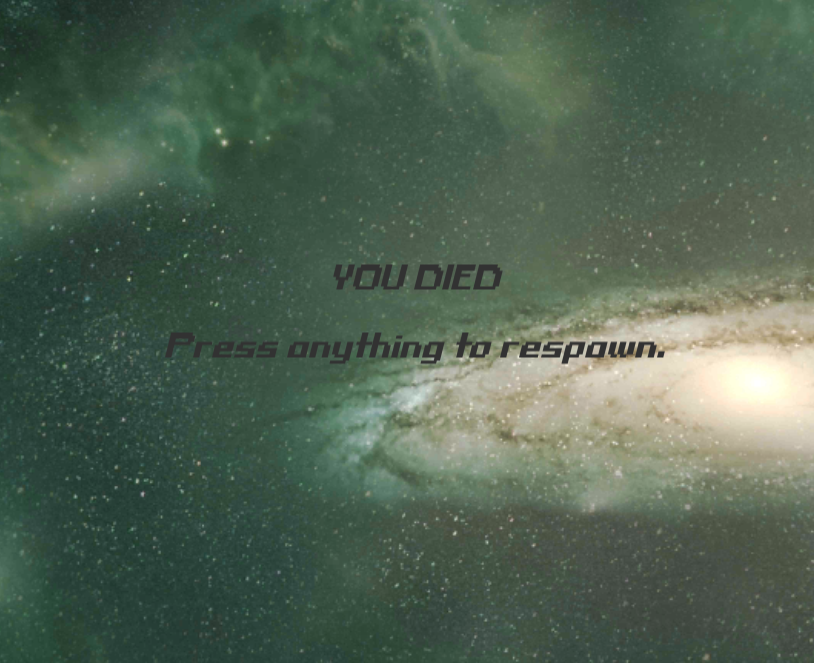
\includegraphics[width = \textwidth, height=\textwidth]{images/game4}
\caption{Defeat screen}
\label{fig:bottom}
\end{subfigure}

\label{fig:right}
\end{subfigure}
\caption{Space Shooter in a nutshell}
\label{fig:combined}
\end{figure}
As depicted in Figure 3, these are the main entities of the Space Shooter. The player ship (c) flies through a field of asteroids (b) as the space drones (a) attempt to destroy the ship. In case of defeat, the game ends and the player is shown the defeat screen (d) with the option of restarting the game.